% !TeX spellcheck = italian
\documentclass[12pt,italian]{report}
\usepackage{tesi}

\usepackage[a4paper]{geometry}		% Formato del foglio
\usepackage[italian]{babel}			% Supporto per l'italiano
\usepackage[utf8]{inputenc}			% Supporto per UTF-8
%\usepackage[a-1b]{pdfx}				% File conforme allo standard PDF-A (obbligatorio per la consegna)

\usepackage{graphicx}				% Funzioni avanzate per le immagini
\usepackage{hologo}					% Bibtex logo with \hologo{BibTeX}
\usepackage{epsfig}				    % Permette immagini in EPS
\usepackage{xcolor}                 % Gestione avanzata dei colori
\usepackage{amssymb,amsmath,amsthm} % Simboli matematici
\usepackage{listings}				% Scrittura di codice
\usepackage{url}					% Visualizza e rendere interattii gli URL
\usepackage[pdfa]{hyperref}			% Rende interattivi i collegamenti interni
\usepackage{tikz}                   % Permette di disegnare inline
\usepackage{import}
\usepackage{float}
\usepackage{xstring}                % Permette di usare la funzione \IfInteger
\usepackage{array}                  % Permette di usare colonne "m" dentro table
\usepackage{multirow}               % Permette di creare tabelle con righe multiple
\usepackage{caption}                % Roba per le figure side-by-side
\usepackage{subcaption}             % Roba per le figure side-by-side
\graphicspath{{immagini/}}

\usetikzlibrary{positioning}
\usetikzlibrary{calc}
\usetikzlibrary{shapes}

\usepackage[autostyle = false]{csquotes}
\MakeOuterQuote{"}

\newcommand{\GeneraSchemaPacchetto}[2]{{
\begin{tikzpicture}
    [
        box/.style={draw,rectangle,minimum width=\recminwidth, 
        minimum height=\rectangleheight, 
        outer sep=0pt, node distance=0pt}
    ]

    \def\rectangleheight{1cm}
    \def\recminwidth{2cm}

    \foreach \name/\size in {#1} {
        \node[box, label={below:\small \texttt{\size{} byte}}] (0) {\texttt{\name}};
    }    

    \foreach \name/\size [count=\i] in {#2}
    {
        \pgfmathtruncatemacro\prevposition{\i - 1}
        \node[box, right = 0pt of \prevposition,
            label={below:\small \texttt{\IfInteger{\size}{\size\ byte}{\size}}}
        ] (\i) {\texttt{\name}};
    }
\end{tikzpicture}
}}

\def\myCDL{Corso di Laurea in\\ Sicurezza dei Sistemi e delle Reti Informatiche}

% TITOLO TESI:
\def\myTitle{VirTEE: implementazione di un protocollo per la condivisione TEE in Cloud}

% AUTORE:
\def\myName{Massimo Perego}
\def\myMat{Matr. Nr. 965229}

% RELATORE E CORRELATORE: 
\def\myRefereeA{Prof. Andrea Lanzi}

% ANNO ACCADEMICO
\def\myYY{2022-2023}

% Il seguente comando introduce un elenco delle figure dopo l'indice (facoltativo)
%\figurespagetrue

% Il seguente comando introduce un elenco delle tabelle dopo l'indice (facoltativo)
%\tablespagetrue

\begin{document}

	\frontespizio
	\afterpreface

	\chapter*{Sommario}
	\addcontentsline{toc}{chapter}{Sommario}  
	\label{cap:sommario}
	
	\chapter{Introduzione}
	\label{sec:introduzione}
	
	\chapter{Trusted Execution Environment}
	\label{cap:TEE}
	Un \textit{Trusted Execution Environment} (TEE) è un'area isolata e sicura all'interno di un dispositivo, concepita con l'intento di operare in modo affidabile ed indipendente dal resto del sistema operativo. Questo permette di ospitare applicazioni e processi sensibili, eseguendo unicamente codice autenticato.
	
	I TEE stanno progressivamente guadagnando maggiore rilevanza in virtù del loro impiego per l'arricchimento di piattaforme preesistenti, offrendo soluzioni atte a incrementare la sicurezza e prevenire accessi o manipolazioni non autorizzate. Grazie a tali caratteristiche, i TEE trovano utilizzo in diverse applicazioni e ambiti operativi.
	
	\bigbreak
	
	I TEE sono presenti sulla maggioranza dei cellulari tramite nomi quali \textit{TrustZone} di ARM, \textit{Samsung Knox}, \textit{Qualcomm QTEE}, \textit{Google Titan M} e \textit{Apple Secure Enclave}, con più finalità, tra le quali: autenticazione sicura, gestione di chiavi crittografiche e gestione dei diritti digitali.
	
	L'impiego dei TEE però sta assumendo un ruolo crescentemente significativo non solo nell'ambito dei dispositivi mobili, ma anche nei settori Desktop, Server e IoT. Sono sempre più numerosi i prodotti sul mercato che consentono esecuzione di codice sicuro anche in tali ambienti. Tale tendenza riflette la crescente preoccupazione per la sicurezza informatica e la protezione dei dati sensibili in un'ampia gamma di applicazioni e scenari operativi.
	
	In questo capitolo verranno esplorate le principali caratteristiche dei TEE e come tali implementazioni possano contribuire a migliorare l'affidabilità di vari tipi di sistemi.
	
	\newpage
	
	\section{TEE GlobalPlatform}
	\label{sec:GlobalPlatform}
	%Deve contenere: cos'è globalplatform, architettura, cosa ne consegue (che sicurezza e cosa forniscono)
	Il concetto di "Trusted Execution Environment" denota una combinazione di tecniche software e hardware progettate per creare un ambiente sicuro e protetto. Nonostante ciò, il termine risulta piuttosto generico, in quanto fa riferimento a una vasta gamma di prodotti con caratteristiche implementative e livelli di sicurezza diversi.
	
	L'assenza di standardizzazione potrebbe essere causa di confusione tra i consumatori e diventare un ostacolo per la portabilità ed interoperabilità di Trusted Applications (TA) su diverse implementazioni di TEE. Ciò implica la necessità di gestire una gamma di differenze nell'implementazione e garanzie di sicurezza offerte, complicando l'utilizzo di tali ambienti in modo uniforme e trasversale.
	
	A risoluzione di questi problemi il consorzio GlobalPlatform pubblica dei documenti contenenti specifiche che coprono vari aspetti chiave della realizzazione di TEE, favorendo l'interoperabilità tra dispositivi e sistemi.
	
	All'interno delle specifiche di GlobalPlatform, si possono trovare direttive dettagliate relative a diverse tematiche riguardanti i Trusted Execution Environments, tra le quali: il modello architetturale dei TEE, delineando le sue componenti fondamentali, un insieme standard di interfacce API e metodi per la gestione sicura delle credenziali.
	
	\bigbreak
	
	Un altro aspetto trattato è l'istituzione di parametri e criteri per la valutazione della sicurezza dei TEE. Attraverso queste direttive, si mira a garantire che tali ambienti protetti soddisfino precisi standard di robustezza e affidabilità.
	
	Un numero sempre crescente di organizzazioni sta adottando questi standard e adeguando le proprie soluzioni alle specifiche GlobalPlatform. La tendenza generale è di una sempre più ampia adozione di TEE in conformità con queste direttive, pertanto questo elaborato farà riferimento a TEE conformi GlobalPlatform.
	
	\bigbreak 
	
	In generale, l'implementazione di un TEE conforme alle direttive di GlobalPlatform consente di garantire un elevato livello di sicurezza, interoperabilità e affidabilità del TEE su una vasta gamma di dispositivi e piattaforme, creando un ambiente di esecuzione sicuro per applicazioni sensibili e riservate.
	
	\newpage
	
	\subsection{Architettura TEE}
	\label{subsec:architettura}
 	Le direttive di GlobalPlatform non fanno riferimento ad implementazioni specifiche per quanto riguarda l'architettura, ma piuttosto delineano una struttura generale degli elementi logici costituenti il TEE e le loro interazioni. Vengono solamente stabiliti i requisiti di sicurezza che l'hardware deve poter garantire al TEE.
 	
 	\bigbreak
 	
 	In generale, il sistema è suddiviso in due ambienti distinti, noti come \textit{Trusted Execution Environment} (TEE) e \textit{Regular Execution Environment} (REE). Quest'ultimo costituisce l'insieme dei componenti di un dispositivo e il sistema operativo convenzionale. Generalmente si ha un solo TEE, ma nulla vieta di implementarne molteplici, sebbene si tratti di una pratica poco comune. Da qui in poi si farà riferimento ad un ambiente con un solo TEE e REE per semplicità.
 	
 	Ogni risorsa può essere controllata dal REE o da un TEE ed il possesso può essere trasferito tra gli ambienti. Una risorsa controllata da uno specifico TEE viene isolata dagli altri ambienti di esecuzione, se non altrimenti specificato esplicitamente dal TEE. In generale, il TEE può avere capacità di accedere alle risorse del REE, mentre il contrario non è possibile, a meno che non siano concessi permessi specifici. 
 	
 	L'unico modo che il REE ha per accedere alle risorse in ambiente protetto è tramite entry point delle API o servizi esposti dal TEE, ma non viene specificato un metodo preciso per imporre il controllo degli accessi.
 	
 	\begin{figure}
 		\centering
 		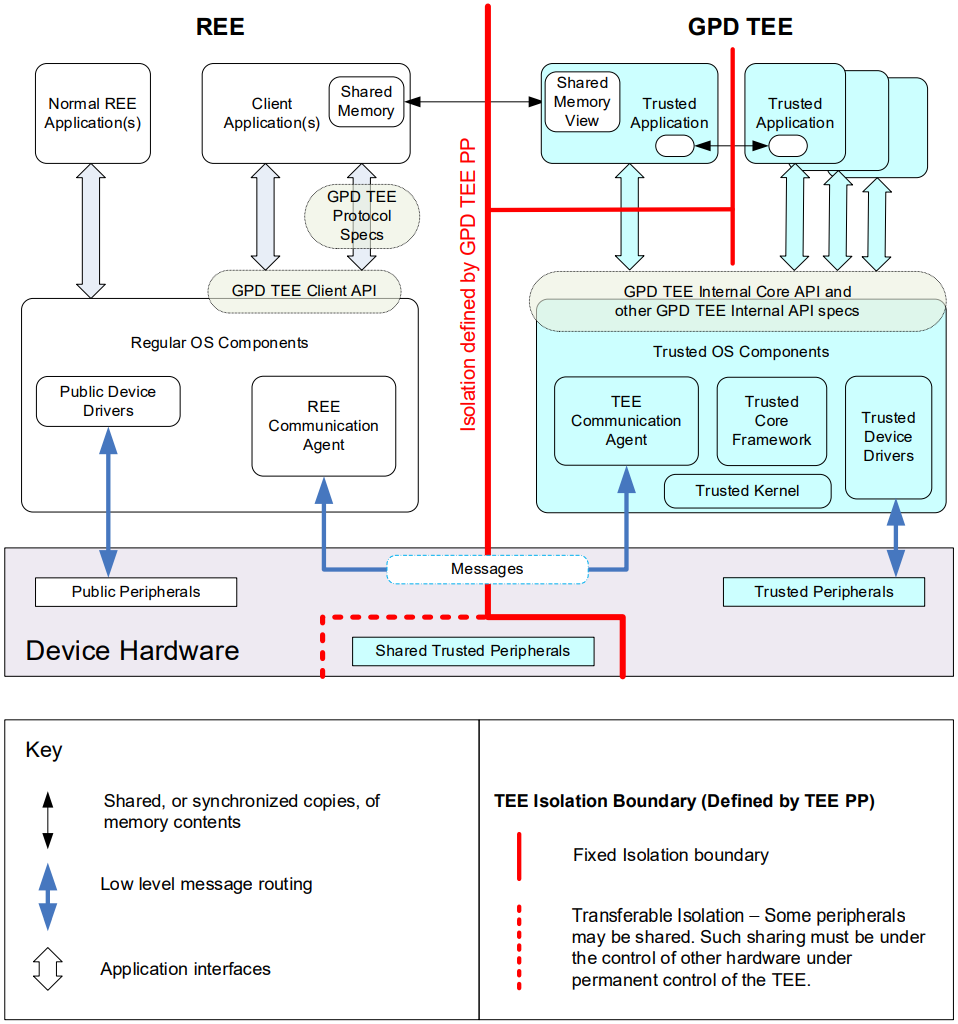
\includegraphics[width=1\textwidth]{immagini/TEE_SW_Architecture}
 		\caption{
 			Architettura di un TEE conforme GlobalPlatform. 
 			Da \textit{TEE System Architecture v1.3 (pag. 28)}
 			\cite{gp2020systemarchitecture}
 		}
 		\label{fig:tee-architecture}
 	\end{figure}
 	
 	\bigbreak
 	
 	In \figurename~\ref{fig:tee-architecture} si può vedere un possibile esempio di architettura software di un sistema conforme GlobalPlatform. Si può vedere la separazione di REE e TEE, in quanto ambienti completamente separati, dotati ciascuno di sistema operativo, scheduling e risorse proprie.
 	
 	Le applicazioni all'interno del REE vengono classificate come \textit{Client Applications} (CA), mentre le applicazioni all'interno del TEE sono denominate \textit{Trusted Applications} (TA).
 	
 	All'interno del TEE è presente un \textit{Trusted Kernel} che fornisce scheduling ed altre funzioni di gestione del sistema operativo, sia per le TA che per il Trusted Core Framework.
 	
 	\bigbreak
 	
 	Una CA per richiedere un servizio da una Trusted Application utilizza la \textit{Client API}. Tale API consente di stabilire una sessione con la TA e inviare un messaggio contenente la funzione da invocare e i relativi parametri.
 	
 	All'interno di entrambi gli ambienti sono presenti dei \textit{Communication Agent}. Questi agenti si occupano di fornire il supporto per lo scambio di messaggi tra la Client Application e la Trusted Application e, se necessario, anche tra diverse TA.
 	
 	
 	\paragraph{Trusted Core Framework:} le Trusted Application possono fare uso della \textit{Trusted Core Framework API}, la quale definisce API ed infrastrutture simili a quelle presente in un sistema operativo. Ciò permette di avere un'interfaccia comune per le TA, indipendentemente dal TEE sulla quale vengono eseguite. Queste specifiche sono contenute all'interno del \textit{TEE Internal Core API Specification}\cite{gp2020internalapi}.
 	
 	\paragraph{Periferiche:} vengono suddivise in tre categorie: 
 	\begin{itemize}
 		\item \textit{Public Peripherals}: possono essere utilizzate sia dal TEE che dalle applicazioni REE. L'accesso dalle TA avviene attraverso API fornite dal TEE. L'utilizzo da parte di applicazioni esterne al TEE segue le modalità di accesso standard del sistema operativo.
 		\item \textit{Trusted Peripherals}: l'accesso a questo periferiche è consentito esclusivamente a TA autorizzate, tramite interfacce API definite dal TEE.
 		\item \textit{Shared Trusted Peripherals}: di norma l'accesso a queste periferiche è consentito solo al TEE, ma questo può concedere temporaneamente l'accesso anche al REE. Il processo di condivisione deve essere comunque gestito da hardware sotto il controllo del TEE.
 	\end{itemize}
 	
 	
 	\subsection{Garanzie di Sicurezza}
 	\label{subsec:garanzie}
 	Come già detto in precedenza, il termine "Trusted Execution Environment" può fare riferimento ad una moltitudine di prodotti, quindi questi potrebbero variare in termini di garanzie di sicurezza che forniscono. Per questo motivo GlobalPlatform ha definito all'interno del \textit{Protection Profile} \cite{gp2020protectionprofile} i requisiti minimi di sicurezza che un TEE deve avere per poter essere certificato. Nonostante le proprietà indicate rappresentino una linea base minima, non è detto che un TEE non possa implementarne altre.
 	
 	\bigbreak
 	
 	In generale si può affermare che un TEE dovrebbe garantire le proprietà di integrità e confidenzialità del codice e di ciò che esso crea, e garantire esecuzione isolata rispetto al REE.
 	
 	Come già visto per altri documenti, GlobalPlatform non stabilisce implementazioni precise ma fornisce solo delle direttive. Nonostante ciò, all'atto pratico si hanno alcune caratteristiche comuni alla maggior parte dei TEE, come l'utilizzo di firme digitali per l'autenticazione del codice e l'utilizzo di supporto hardware per realizzare l'isolamento.
 	
 	\bigbreak
 	
 	\paragraph{Isolamento:} la separazione del sistema in zone isolate al fine di garantire la proprietà di isolamento non è nuova, in quanto già proposta da J.M. Rushby nel 1981 \cite{rushby1981separationkernel}. 
 	
 	Rushby infatti metteva in evidenza come un sistema distribuito permetta di gestire la sicurezza tramite separazione fisica delle parti e mediazione di funzioni fidate.
 	
 	Questo concetto può essere esteso ad una singola macchina, la quale viene vista come sistema distribuito di componenti indipendenti, i quali quindi permettono di ritenere le proprietà di sicurezza di un sistema distribuito.
 	
 	Nel mondo TEE questa idea viene ripresa tramite l'implementazione di un \textit{separation kernel}, l'elemento usato per simulare un sistema distribuito, come evidenziato da Sabt et al \cite{sabt2015tee}. Questo permette la coesistenza di diversi sistemi, con diversi requisiti di sicurezza, sulla stessa piattaforma. Fondamentalmente divide il sistema in partizioni e garantisce isolamento tra di esse, tranne per alcune interfacce controllate.
 	
 	I requisiti di sicurezza generali del separation kernel si possono trovare all'interno del \textit{Separation Kernel Protection Profile} (SPKK) \cite{spkk2007}, ma si possono riassumere in quattro policy di sicurezza principali: 
 	\begin{itemize}
 		\item \textit{Data (spatial) separation:} dati all'interno di una partizione non possono essere letti o modificati da altre partizioni.
 		\item \textit{Sanitization (temporal separation):} le risorse condivise non devono permettere la fuoriuscita di informazioni ad altre partizioni.
 		\item \textit{Control of information flow:} la comunicazione tra partizioni deve sempre essere espressa esplicitamente.
 		\item \textit{Fault isolation:} falle di sicurezza in una partizione non devono poter condizionare le altre.
 	\end{itemize}
 	
 	La separazione di servizi importanti e dati sensibili permette di minimizzare la possibile superficie d'attacco di un sistema, in quanto la compromissione di un componente non causa danni alle altre parti del sistema. L'unica eccezione sarebbe un fallimento del separation kernel stesso, che per questo motivo deve rimanere più semplice possibile. 
 	
 	Nella pratica il sistema distribuito descritto da Rushby si compone di due sole componenti, REE e TEE, in quanto tutte le implementazioni effettive prevedono un solo TEE.
 	
 	\newpage
 	
 	\paragraph{Integrità e autenticità:} i benefici di protezione durante l'esecuzione dati dall'isolamento vengono annullati se non sono garantite integrità ed autenticità del codice, in quanto modifiche a dispositivo spento permetterebbero la compromissione del sistema.
 	
 	\bigbreak
 	
 	Per effettuare questa verifica è necessario un \textit{TEE Secure Boot}, come definito dal \textit{TEE System Architecture} \cite{gp2020systemarchitecture}. Questo è un processo di autenticazione di tutto il software che andrà dentro al TEE, ad eccezione del primissimo codice eseguito per il boot, scritto su una memoria ROM, impossibile da sovrascrivere, la cui integrità è quindi intrinsecamente garantita.
 	
 	\bigbreak
 	
 	Ogni componente caricato permette di verificare e caricare il componente successivo, come mostrato in \figurename~\ref{fig:tee-secure-boot}. La verifica può essere implementata, ad esempio, tramite un meccanismo di autentecazione basato su coppie di chiavi, che permettono di firmare e verificare l'hash del codice da caricare. Questo permette di garantire che un ente fidato abbia approvato quel software.
 	
 	Il firmware del dispositivo deve però conoscere le chiavi pubbliche necessarie per poter verificare la firma dei software da caricare, ma si tratta di un dettaglio implementativo dipendente dal sistema.
 	
 	\bigbreak
 	
 	Prima di uscire dal processo di boot il firmware può verificare il boot loader del REE prima della sua esecuzione. In caso di fallimento di verifica di qualsiasi dei componenti prima di questo generalmente il dispositivo termina il processo e viene riavviato, altrimenti continua con l'esecuzione del REE boot loader.
 	
 	\bigbreak
 	
 	Questo processo non è dissimile da quello di un \textit{Secure Boot} tradizionale, con le differenze che in un TEE questo processo non termina con l'avvio del sistema operativo e non verifica solo il processo, ma anche il software che andrà in esecuzione sul sistema.
 	
 	\begin{figure}
 		\centering
 		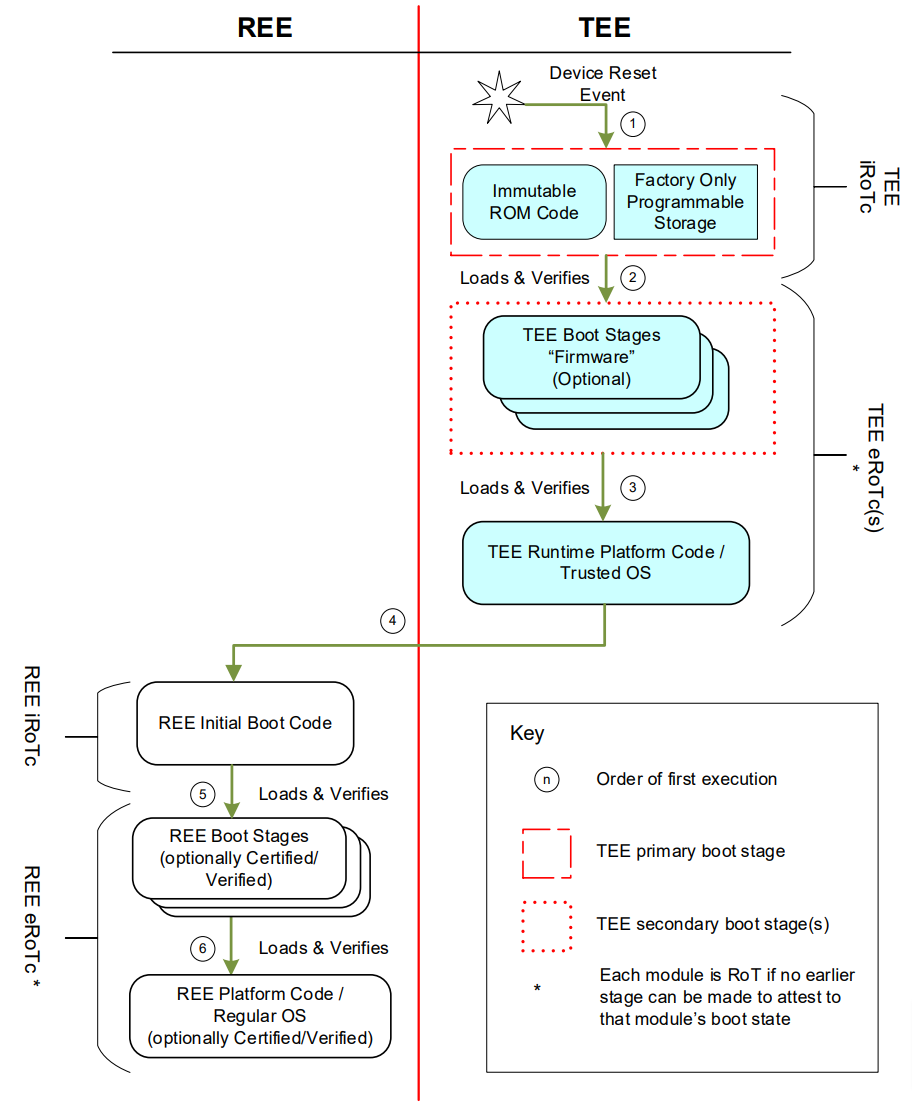
\includegraphics[width=1\textwidth]{immagini/TEE_Secure_Boot}
 		\caption{
 			Esempio di TEE Secure Boot. 
 			Da \textit{GlobalPlatform TEE System Architecture pag. 73}
 			\cite{gp2020systemarchitecture}
 		}
 		\label{fig:tee-secure-boot}
 	\end{figure}
 	
 	\newpage
 	
 	\section{Applicazioni dei TEE}
 	\label{sec:applicazioni}
	I Trusted Execution Environment, grazie alle proprietà di sicurezza che garantiscono, permettono lo sviluppo di nuove applicazioni prima non possibili e l'espansione di quelle già esistenti.
	
	Fino ad ora la maggiore diffusione dei TEE è rimasta in ambito mobile, anche se non sempre pubblicizzati esplicitamente. L'utilizzo non è però limitato a questo settore, le applicazioni dei TEE possono essere molteplici, anche se la maggioranza dei dispositivi non permette l'installazione di software all'interno del TEE dopo la configurazione iniziale.
	
	\bigbreak
	
	Però, tramite l'adozione sempre più vasta degli standard GlobalPlatform e lo sviluppo di TEE open-source come OP-TEE \cite{optee}, si ha una crescente tendenza ad aprire la possibilità a più sviluppatori di implementare i propri TEE e permettere un uso sempre più vasto di questa tecnologia da parte di tutti.
	
	
	\subsection{Archiviazione Sicura}
	\label{subsec:secure-storage}
	Una delle applicazioni più comuni dei TEE è il secure storage, ovvero un meccanismo che consente di proteggere e preservare dati sensibili e critici all'interno di un ambiente altamente affidabile e isolato. Il TEE fornisce una zona sicura all'interno del dispositivo in cui i dati possono essere memorizzati e gestiti in modo sicuro, garantendo la privacy e la riservatezza delle informazioni.
	
	Vengono spesso utilizzati per memorizzare sui dispositivi mobili elementi quali chiavi crittografiche, credenziali di autenticazione, certificati digitali, informazioni finanziarie ed altri dati personali.
	
	\bigbreak
	
	L'implementazione Android del secure storage è \textit{Android Keystore} \cite{androidkeystore}, che fa ampio uso del sistema \textit{Trusty TEE} \cite{androidtrustytee}, basato su ARM TrustZone. Questo sistema offre una API per gestire in modo sicuro e protetto le chiavi e i certificati all'interno del TEE, in modo da permettere alle applicazioni di usarlo per operazioni di crittografia, firma digitale e autenticazione.
	
	Inoltre, il sistema Android Keystore offre funzionalità avanzate, come la generazione delle chiavi direttamente all'interno del TEE, senza mai esporre le chiavi al sistema operativo principale. 
	
	\bigbreak
	
	GlobalPlatform ha definito delle specifiche per la gestione del secure storage, ovvero il \textit{Secure Element Access Control} \cite{gp2020seac}, stabilendo un framework standardizzato per la gestione e protezione dati all'interno del TEE. Un'implementazione comune prevede l'utilizzo di chiavi crittografiche generate e archiviate all'interno del TEE, le quali vengono utilizzate per crittografare i dati sensibili e per proteggere l'accesso al secure storage.
	
	\bigbreak 
	
	Inoltre ci sono alcune implementazioni di \textit{Trusted Platform Module} (TPM) all'interno dei TEE, tramite la funzionalità del Secure Storage. Normalmente il TPM costituisce un componente hardware distinto dal resto del sistema, concepito con obiettivi quali la generazione e la conservazione di chiavi crittografiche, la firma e l'autenticazione sicure, nonché la misurazione dell'integrità del sistema.
	
	Le caratteristiche fisiche e le garanzie di sicurezza offerte da un TPM risultano quindi analoghe a quelle precedentemente descritte per un TEE, mentre l'integrazione del TPM all'interno di quest'ultimo consente di evitare il costo dell'hardware tipicamente richiesto per un chip TPM indipendente.
	
	\subsection{Protezione Contenuti Multimediali (DRM)}
	\label{subsec:drm}
	Nell'era digitale, l'accesso, la distribuzione e la protezione dei contenuti digitali sono diventati elementi cruciali per le industrie dell'intrattenimento, dei media e delle comunicazioni. Tuttavia, con l'aumento della pirateria e delle violazioni dei diritti d'autore, è diventato essenziale sviluppare soluzioni di Digital Rights Management (DRM) sempre più sofisticate per garantire la sicurezza dei contenuti e proteggere i diritti dei creatori e dei detentori dei contenuti stessi.
	
	\bigbreak
	
	Per questo motivo l'utilizzo di sistemi come \textit{Widevine} \cite{widevine} e \textit{PlayReady} \cite{playready} permette di sfruttare l'ambiente TEE (con il loro più alto livello di protezione) per funzionalità quali cifratura del flusso video, verifica delle licenze digitali, autenticazione del dispositivo e protezione contro la copia non autorizzata. Permette anche di mostrare a schermo il video senza che altre applicazioni esterne al TEE possano leggerne i contenuti, a patto che sia presente un canale di comunicazione fidato tra TEE e display, quindi indipendente dal resto del sistema.
	
	Questo permette di garantire che i contenuti video siano accessibili solo da dispositivi e applicazioni autorizzati, proteggendo così i diritti dei detentori dei contenuti e i loro partner di distribuzione. 
	
	\subsection{Garanzie di Sicurezza nel Cloud Computing}
	\label{subsec:protezione-cloud}
	Il cloud computing è un modello di erogazione servizi informatici il quale consente l'accesso on-demand a tramite Internet, senza la necessità di gestire fisicamente l'infrastruttura e sfruttando le risorse richieste in modo estremamente efficiente e scalabile.
	
	Con questo modello sorgono però altre problematiche di sicurezza; ad esempio, il cloud provider deve poter gestire la macchina in quanto mantenitore dell'infrastruttura, ma questo significa anche che ha la capacità di poter leggere tutti i dati presenti in memoria.
	
	Inoltre un elemento fondamentale alla scalabilità del modello è l'utilizzo di una sola macchina fisica per molteplici macchine virtuali (VM), possibilmente assegnate ad altrettanti clienti. Questo significa che più clienti condividono la stessa memoria fisica, aprendo la porta a possibili attacchi che eludono le misure messe in atto per l'isolamento di una VM dalle altre, come già successo \cite{vmescape1} \cite{vmescape2} \cite{vmescape3}. In questo modo gli attaccanti avrebbero modo di accedere ai dati presenti all'interno delle altre macchine virtuali ed in alcuni casi anche di manipolareil codice per i loro scopi.
	
	\bigbreak
	
	In un tale ambiente è normale che un'organizzazione possa ricercare metodi per garantire che il codice eseguito in remoto sia effettivamente quello desiderato. I TEE permettono di implementare sistemi di attestazione remota del codice, generalmente realizzati tramite una TA o meccanismi hardware che generano un report firmato digitalmente sullo stato di esecuzione della macchina. La chiave privata rimane solamente all'interno del TEE, garantendone la sicurezza.
	
	\subsection{Altri Usi}
	\label{subsec:altri-usi}
	Oltre alle applicazioni precedentemente menzionate, i TEE hanno stimolato proposte e trovato impieghi in una vasta gamma di settori, abbracciando un'ampia varietà di utilizzi e applicazioni.
	
	\bigbreak
	
	Nel mondo IoT ci sono state proposte decentralizzare la gestione dei dati utilizzando TEE e smart contract \cite{iotblockchain}. L'idea è quella di un sistema in cui i permessi di accesso vengono applicati tramite smart contract, memorizzando la cronologia di eventi di accesso ai dati nella blockchain. In questo modo le interazioni non necessitano di un sistema centralizzato, in quanto gli smart contract permettono a più parti di specificarne le regole. Infine fornisce un framework che memorizza l'hash dei dati nella blockchain e archivia i dati grezzi all'interno del TEE.
	
	\bigbreak
	
	Un altro esempio è l'implementazione di un protocollo Vehicle-to-Vehicle (V2V) che permette di fornire autenticazione, privacy e resistenza alla manomissione ad i collegamenti tra veicoli a guida autonoma \cite{teeuses_vehicles}. In questo modo, tramite l'utilizzo dei TEE, si previene l'intercettazione e manomissione dei dati, pur mantenendo l'efficienza e scalabilità necessarie per un sistema tale.
	
	\newpage
	
	\section{Implementazioni Hardware per i TEE}
	\label{sec:supporto-hw}
	Affinché un TEE possa soddisfare le proprietà di sicurezza necessarie, è fondamentale che esso disponga di un supporto hardware adeguato. Ad esempio, un requisito critico che necessita tale sostegno è la proprietà di isolamento rispetto al resto del sistema.
	
	Esistono moltemplici soluzioni per implementare queste proprietà, perciò in questo capitolo verranno esplorate brevemente alcune delle principali proposte sul mercato.
	
	\subsection{Intel SGX}
	\label{subsec:sgx}
	Intel Software Guard Extensions (SGX) è un'estensione dell'architettura x86 sviluppata da Intel per introdurre un ambiente di esecuzione protetto all'interno dei processori. Viene introdotta nel 2015 con la sesta generazione di processori Intel Core.
	
	SGX consiste in un insieme di istruzioni hardware e strutture di memoria che consentono la creazione e l'isolamento di \textit{enclavi} sicure all'interno del processore, ovvero zone di memoria di dimensione ridotta crittografate e protette tramite meccanismi hardware. 
	
	Per l'accesso a queste zone di memoria è necessario utilizzare i nuovi metodi introdotti da SGX, come ad esempio l'istruzione \texttt{ECREATE} permette di creare un'istanza di enclave, mentre l'istruzione \texttt{ECALL} consente alle applicazioni di interagire con il codice all'interno dell'enclave in modo controllato e sicuro. 
	
	Le istruzioni introdotte sono comparabili a quelle per il passaggio da user mode a kernel mode. Le enclavi vengono sempre eseguite al ring 3 di privilegio (il più basso) ed utilizzano la traduzione degli indirizzi fornita da kernel e hypervisor.
	
	\bigbreak
	
	Come descritto da \cite{sgx_explained}, all'avvio del sistema SGX riserva una porzione di memoria designata come \textit{Processor Reserved Memory} (PRM). Tale area di memoria risulta inaccessibile a tutte le richieste di accesso che non sono riconducibili a un contesto di enclave. Questo ambito di restrizione si estende anche ad elementi quali kernel, hypervisor, System Management Mode (SMM) e Direct Memory Access (DMA).
	
	All'interno di questa zona di memoria si possono trovare la \textit{Enclave Page Cache} (EPC), ovvero pagine di 4KB contenenti codici e dati delle enclavi, oltre all'\textit{Enclave Page Cache Map} (EPCM), la quale viene utilizzata dalla CPU per tracciare lo stato delle pagine all'interno dell'EPC, permettendo di garantire che ciascuna pagina appartenga ad una sola enclave. Quest'ultima è sempre inaccessibile, indipendentemente dal livello di privilegio.
	
	\bigbreak
	
	Un'enclave viene creata tramite l'istruzione \texttt{ECREATE}, la quale inserisce in una pagina libera dell'EPC la \textit{SGX Enclave Control Structure} (SECS). Quest'ultima andrà a contenere informazioni di controllo e metadati relativi all'enclave stessa, come dimensione, base address ed altre proprietà. L'identità di un'enclave è strettamente legata alla sua SECS, in quanto la entry che identifica l'enclave all'interno della EPCM punta alla SECS della stessa. Il sistema usa l'indirizzo virtuale della SECS per identificare l'enclave quando vengono utilizzate istruzioni di SGX.
	
	In seguito il sistema utilizza l'istruzione \texttt{EADD} per caricare codice e dati iniziali all'interno dell'enclave. I dati vengono letti da una struttura chiamata \textit{Page Information} (PAGEINFO), la quale contiene l'indirizzo della pagina EPC da allocare e l'indirizzo della pagina sorgente che andrà copiata nella EPC.
	
	In seguito ad aver caricato i dati necessari, il sistema deve usare una \textit{Launch Enclave} (LE) per ottenere una \textit{EINIT Token Structure}. Tramite l'istruzione \texttt{EINIT} ed il token generato la SECS in questione viene segnata come inizializzata.
	
	Alla fine del processo di vita di un'enclave l'istruzione \texttt{EREMOVE} permette la deallocazione delle pagine utilizzate dall'enclave all'interno della ECP.
	
	La LE è un'enclave privilegiata fornita da Intel, firmata con una chiave presente nell'implementazione di SGX quindi esente dal richiedere un EINIT Token. Questa permette di verificare l'identità di un'enclave in fase di creazione e necessita di informazioni quali chiave di crittografia dell'enclave, politiche di protezione, ecc.
	
	\bigbreak
	
	A partire dai processori di undicesima e dodicesima generazione Intel SGX è stato deprecato sui processori Intel Core, ma continua lo sviluppo per i processori Xeon, comunemente utilizzati in ambito cloud e server.
	
	\subsection{AMD SEV}
	\label{subsec:sev}
	AMD Secure Encrypted Virtualization è una tecnologia introdotta nel 2016 come estensione dell'architettura x86 progettata per offrire isolamento per la memoria di macchine virtuali (VM). Anche se comunemente l'hypervisor viene considerato un componente fidato nel modello di sicurezza della virtualizzazione, tuttavia può non essere sempre così, come ad esempio in ambiente cloud, dove i clienti potrebbero volere una maggiore confidenzialità dei loro dati, normalmente accessibili al service provider.
	
	Al fine di risolvere questo problema AMD SEV permette di crittografare in modo granulare la memoria associata a una specifica macchina virtuale, conferendole un livello di inaccessibilità anche per l'hypervisor stesso. Ogni VM possiede la sua chiave di crittografia unica. La cifratura dei dati in memoria è affidata ad un chip hardware AES-128. Esiste la possibilità da parte della VM di condividere determinate pagine con l'hypervisor.
	
	In aggiunta, sulla scheda madre, trova posto un processore ARM denominato \textit{Secure Processor} (SP), contenente un firmware proprietario. Questo componente assume responsabilità diverse, tra cui la gestione delle chiavi crittografiche. Inoltre fornisce delle API che l'hypervisor deve utilizzare per gestire le chiavi.
	
	\bigbreak
	
	Il SP permette anche un processo di attestazione remota, per aver modo di verificare che le VM in esecuzione presenti in un ambiente remoto siano effettivamente quelle desiderate e che queste siano all'interno dell'ambiente corretto. Viene generato un report contenente tutte le informazioni necessarie per verificarlo, come ad esempio dati iniziali della macchina e policy di sicurezza applicate. In seguito viene firmato tramite una chiave privata presente solamente all'interno del processore, la quale corrispondente pubblica viene fornita da AMD per verificare l'attendibilità del report.
	
	\bigbreak
	
	Partendo da una nuova VM, prima di andare in esecuzione con SEV, questa passa da tre stati, il primo dei quali è UNINIT. In questa fase, con il supporto dell'hypervisor, viene effettuato lo scambio di chiavi con il SP (di tipo ECDH). 
	
	Una volta terminato passa allo stato LUPDATE, nel quale vengono caricati e crittografati i dati da inserire all'interno della VM. Al termine di questo viene calcolato un HMAC per verificare che i dati iniziali non sono stati modificati e passa allo stato LSECRET.
	
	Questo stato permette di passare dati già criptati, quindi che necessitano confidenza più elevata, alla VM. Rimane l'hypervisor come intermediario, che però non può effettuare modifiche/azioni significative con i dati passati. 
	
	Al termine di questo stato la macchina virtuale può andare in modalità di esecuzione regolare.
	
	\bigbreak
	
	In seguito AMD ha rilasciato versioni aggiornate di SEV, la prima delle quali nel 2017: SEV-ES (Encrypted State) \cite{sev_es}, incentrata sulla crittografia dello stato dell'architettura delle CPU, criptando anche registri interni, page table e altre strutture interne. Prima di questo SEV salvava in chiaro i registri di una VM dopo un context switch con l'hypervisor.
	
	Nel 2021 viene rilasciata SEV-SNP (Secure Nested Paging) \cite{sev_snp}, introdotta per migliorare la sicurezza nelle architetture di multi-tenant e cloud. Introduce una nuova tabella di pagine crittografata all'interno di ogni VM che garantisce l'isolamento tra VM diverse. Le VM non possono accedere alle tabelle di pagine l'una dell'altra.
	
	\newpage
	
	\subsection{Arm TrustZone}
	\label{subsec:trustzone}
	ARM TrustZone è una tecnologia di sicurezza introdotta nel 2004 e integrata nei processori ARM, che sono ampiamente utilizzati in dispositivi mobili, dispositivi IoT (Internet of Things) e altri sistemi embedded. L'obiettivo principale di TrustZone è creare un ambiente sicuro all'interno di un singolo processore, in modo che diverse parti del sistema possano operare in modalità sicura o non sicura, a seconda delle esigenze, senza compromettere la sicurezza dei dati e delle operazioni.
	
	TrustZone divide il processore in due mondi distinti: "\textit{Secure}" e "\textit{Non-Secure}", i quali operano in parallelo, con risorse distinte per ogni ambiente e separate in modo hardware. Questo fornisce un ambiente in cui è possibile eseguire software critico e operazioni di sicurezza in modo isolato dal resto del sistema.
	
	All'interno di ARM sono presenti 4 livelli di privilegio, da EL0 (più basso) a EL3 (più alto). Il livello più alto viene utilizzato dal sistema per il passaggio da mondo \textit{Secure} e \textit{Non-secure}. Questo livello rappresenta il \textit{separation kernel} descritto precedentemente (\ref{subsec:garanzie}).
	
	Il software che gestisce il passaggio, sui processori serie Cortex-A, è chiamato "\textit{Secure Monitor}". Sui dispositivi dotati di Cortex-M non è presente in quanto il passaggio da un mondo all'altro è implementato direttamente all'interno della logica del processore. In entrambi i casi si ha una separazione completa e garantita a livello hardware.
	
	\bigbreak
	
	Il processore può trovarsi in solo uno dei mondi e lo stato attuale può essere rilevato tramite un nuovo bit presente sul bus dati, il \textit{Non-Secure} (NS) bit. Quest'ultimo può essere letto tramite il \textit{Secure Configuration Register} (SCR), il quale contiene vari flag e bit che controllano il comportamento del sistema. 
	
	Inoltre il firmware deve implementare un modo per gestire la \textit{Secure Monitor Call} (SMC), l'istruzione che permette di entrare in "\textit{monitor mode}" e cambiare la modalità del processore. Funziona similmente ad una system call: quando chiamata tramite il suo codice specifico passa al livello di privilegio EL3 e invoca un handler implementato nel firmware, all'interno della tabella degli interrupt del processore.
	Il firmware a livello EL3 è anche incaricato di caricare i sistemi operativi del mondo sicuro e normale.
	
	
	\bigbreak
	
	TrustZone estende anche l'infrastruttura di memoria con alcune funzionalità di sicurezza, in particolare: \textit{TrustZone Address Space Controller} (TZASC) e \textit{TrustZone Memory Adapter} (TZMA).
	
	Il TZASC permette partizionare la DRAM e marcare specifiche regioni di memoria come sicure o non-sicure, in modo che applicazioni nel secure world possano accedere alle regioni associate al mondo normale, ma non in contrario. Il TZMA effettua una funzione simile ma su altre memorie come ROM o SRAM.
	
	Queste componenti sono opzionali, quindi la loro presenza e la granularità al quale possono agire dipende dall'implementazione.
	
	\bigbreak 
	
	All'interno di TrustZone non viene effettuata nessuna verifica dell'integrità del codice all'avvio, onere lasciato ai produttori.
	
	Una soluzione comune è avere una coppia di chiavi pubblica e privata, presenti all'interno del chip. Il codice viene caricato assieme ad un suo hash, firmato con la chiave pubblica e poi il tutto viene confrontato con la chiave stampata nel chip.
	
	\begin{figure}[t]
		\centering
		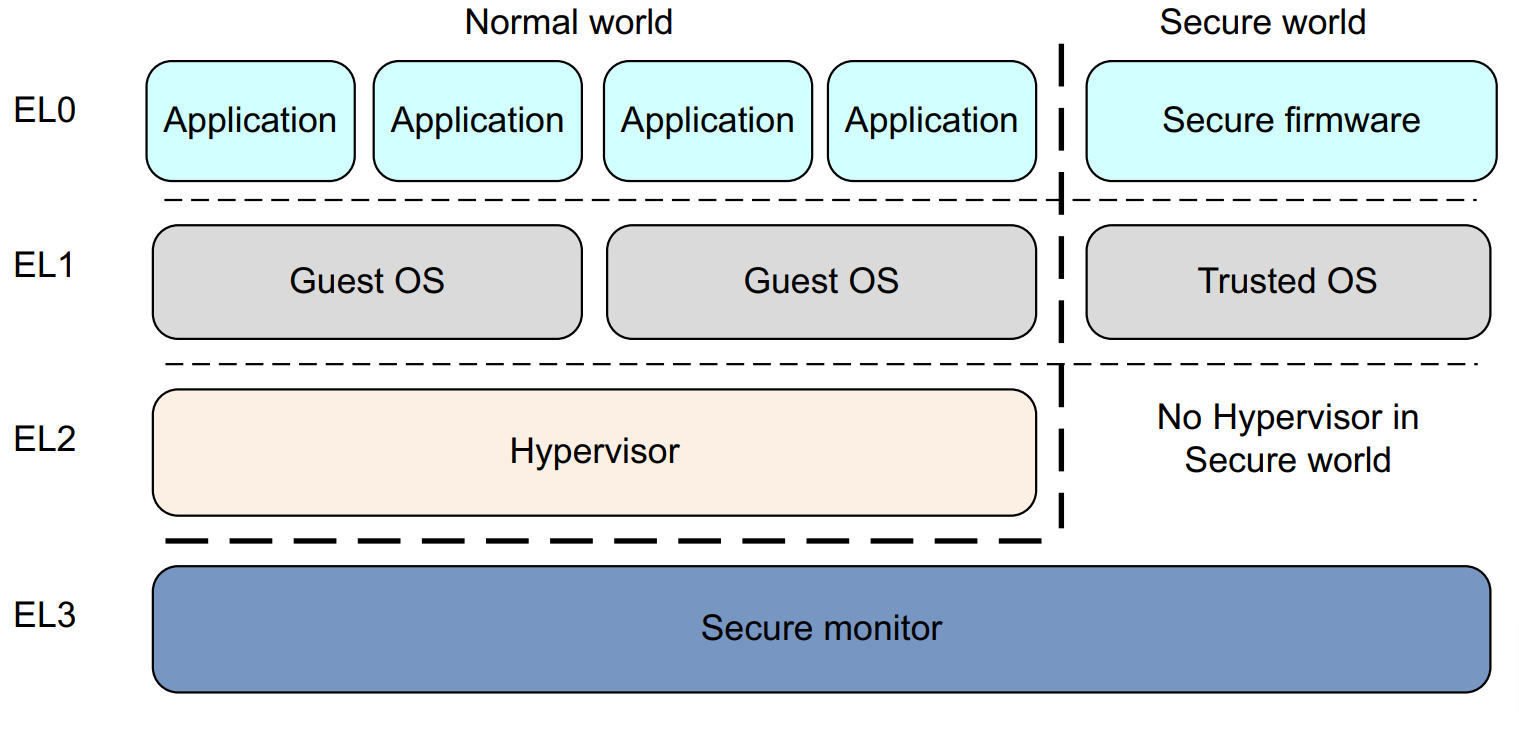
\includegraphics[width=0.8\textwidth]{immagini/ARM_TZ_Levels}
		\caption{
			Livelli di privilegio di ARM TrustZone. Da \textit{"ARM Cortex-A Series Programmer's Guide for ARMv8-A"}
			\cite{arm_programmers_manual}
		}
		\label{fig:arm-exception-levels}
	\end{figure}
	
	\subsection{TEE RISC-V}
	\label{subsec:riscv}
	RISC-V è un Instruction Set Architecture (ISA) sviluppato principalmente dall'Università della California, Berkeley, negli Stati Uniti. Il progetto è nato nel 2010 per poi coinvolgere anche contributori volontari non affiliati all'università. Nel 2015 viene fondata la RISC-V Foundation, creata con il fine di sostenere e promuovere lo sviluppo e l'adozione dell'architettura RISC-V.
	
	Diversamente da molti altri ISA, RISC-V è sviluppato sotto licenza open source, quindi l'utilizzo è gratuito. Questo, oltre al buon supporto da parte di toolchain e sistemi operativi, ha permesso di far crescere notevolmente nel tempo l'adozione di RISC-V, coinvolgendo una vasta comunità di aziende, istituti di ricerca e sviluppatori indipendenti. 
	
	La possibilità di avere a disposizione uno stack software senza doverlo scrivere da zero o pagare licenze ha reso RISC-V un ambiente interessante per sviluppare hardware, anche in ambito TEE.
	
	\bigbreak
	
	Data la flessibilità dell'hardware, i progetti esistenti generalmente si concentrano sulla possibilità di creare TEE che rispondano alle proprie esigenze. Per citare alcuni di questi progetti, Penglai \cite{penglai} e Keystone \cite{keystone}. 
	
	Le soluzioni esistenti, citate nelle sezioni precedenti, pongono limiti progettuali che possono rendere difficoltoso utilizzare l'ambiente in un modo che sia in linea con le proprie esigenze, a volte forzando gli sviluppatori a creare soluzioni alternative, come ad esempio nel caso di dover eseguire applicazioni non modificate all'interno di SGX \cite{grapheneSGX}.
	
	Entrambi i progetti citati precedentemente si basano sullo sfruttare l'isolazione della memoria fornita da RISC-V, chiamata \textit{Physical Memory Protection} (PMP), per ottenere zone di memorie protette da accessi non autorizzati. Utilizzano la \textit{machine mode} (il livello di privilegio più alto di RISC-V) per eseguire un secure monitor con il compito di separare l'ambiente di esecuzione ordinario dalle enclavi sicure create.
	
	L'idea è simile a quelle presentate precedentemente con TrustZone o SGX, ma con minori limiti alla memoria e più possibilità di configurare le enclavi.
	
	\subsection{Processori Dedicati}
	\label{subsec:altri-rpc}
	Un possibile metodo per integrare un TEE all'interno di un dispositivo è quello di avere un secondo processore collegato solamente alle componenti fidate del sistema. Questa soluzione risulta più costosa, ma si hanno alcuni esempi, in particolare su dispositivi mobili di fascia alta.
	
	\bigbreak
	
	A partire dal Pixel 3 Google ha incluso all'interno dei suoi telefoni anche processori della serie \textit{Titan M}, basati sull'architettura RISC-V, i quali sono sistemi a tutti gli effetti, contenenti la propria memoria, RAM, acceleratore crittografico e sistema operativo. L'area TrustZone, anch'essa presente, viene utilizzata solamente come ponte per interagire con il chip \textit{Titan M}.
	
	Alla base, questo processore è stato pensato come metodo per incrementare le misure di sicurezza standard di Android, normalmente affidate ad un TEE presente sul \textit{System on a Chip} (SoC) principale. Permette quindi di immagazzinare dati sensibili come chiavi crittografiche e dati biometrici, oltre che supportare il processo di Secure Boot e validare la versione di Android in esecuzione.
	
	\bigbreak 
	
	Apple include nei propri dispositivi un sottosistema chiamato \textit{Secure Enclave}. Esegue funzionalità simili agli altri TEE, permettendo di implementare funzionalità come \textit{Apple Pay} e \textit{Touch ID}. Si tratta di un SoC che esegue una versione modificata del kernel L4, un sistema molto ridotto, con l'aggiunta di servizi e driver proprietari. Inoltre è collegato a periferiche proprie, accessibili tramite MMIO, come acceleratore crittografico e generatore di numeri casuali.
	
	\section{Vulnerabilità Comuni}
	\label{sec:vulnerabilità}
	Per quanto incentrati sulla sicurezza i TEE non sono completamente esenti da vulnerabilità. Nel tempo sono stati trovati diversi attacchi che permettono di aggirare le misure di sicurezza offerte da questi sistemi.
	
	\bigbreak 
	
	Un primo vettore d'attacco, comune a più soluzioni hardware, coinvolge la cache. Sia SGX che TrustZone e SEV ne sono risultati suscettibili. Nonostante queste soluzioni rendano generalmente inaccessibili i dati tramite metodi convenzionali, la cache non è fisicamente separata dall'ambiente di esecuzione normale. 
	
	
	
	\chapter{TEE in Ambiente Cloud}
	\label{cap:problema}
	Virttee design problems, problema nel portare roba in cloud e come risolverli. Problematiche e come sono state affrontate. Componenti senza implementazione, mettere schemi di funzionamento
	
	\chapter{Sicurezza dei Dati}
	\label{cap:implementazione}
	Nome WIP. Dettagli riguardo all'implementazione, soluzioni tecniche trovate
	%Iniziare con ciò che ha fatto marco? 
	%Section del capitolo prima?
	
	
	\chapter{Analisi Performance}
	\label{cap:dati}
	%Riportare performance generali del sistema, dati di Marco
	%Analisi performance con l'implementazione
	%Commentare i risultati, perché alcuni sono 4% altri 150%
	
	\chapter{Conclusioni}
	\label{cap:conclusioni}
	%Lavori futuri e conclusioni
	
	\bibliographystyle{unsrt}
	\bibliography{bibliografia}
	\addcontentsline{toc}{chapter}{Bibliografia}

\end{document}
